\section{Metodología}

\textbf{Metodología en V}\\
Para el desarrollo del sistema se tomará en cuenta la metodología en V para el desarrollo de software, partiendo de la definición de requerimientos funcionales, técnicos y no funcionales, trazando un plan para el modelado del sistema mediante casos de uso, comprendiendo las limitaciones, identificando el impacto del mismo y previendo posibles cambios. Se hace un diseño del sistema con la ayuda de toda la información recogida sobre requisitos y análisis, donde veremos el sistema de manera modular, tenemos un total de tres módulos, teniendo la ventaja de identificar los errores en una sección específica. Posteriormente el diseño es implementado con el lenguaje de programación elegido para cada modulo, obteniendo programas ejecutables capaces de ofrecer la funcionalidad esperada. A su vez cada modulo va a ser sometida a pruebas para validar el análisis y diseño previamente hecho \citep{Metodologia1}.
\\
Las pruebas de cada nivel son descritas a continuación:

\begin{itemize}

    \item Pruebas unitarias/modulares: estas pruebas comprueban que todas las funcionalidades especificadas en el diseño del componente sean correctas y cubiertas, estas pruebas son realizadas por el desarrollador del componente.
    
    \item Pruebas de integración/interfaz:
    Conforme los módulos son implementados y probados de manera unitaria, se procede a probar su funcionalidad de manera conjunta, estas pruebas están enfocadas a resolver las siguientes supuestos:
    
    \begin{itemize}
        \item Que espera un componente de otro componente, en termino de servicios.
        \item Como es que estos servicios serán solicitados.
        \item Como es que estos servicios serán entregados.
        \item El manejo de errores por condiciones inesperadas.
    \end{itemize}
    
    Las pruebas deben corroborar el correcto funcionamiento de todas las interfaces entre componentes, al tener todos los componentes y sus interfaces terminadas tendremos como resultado el sistema completo, estas pruebas pueden ser realizadas por el desarrollador del componente.
    
    \item Pruebas del sistema: Una vez el sistema ha sido construido, debe ser probado contra las especificaciones del sistema para comprobar que cubra las funcionalidades requeridas.\\
    Esta parte se enfoca en probar el sistema de manera monolítica y debe incluir las pruebas para validar los requerimientos no funcionales.

    \item Pruebas de validación: similar a las pruebas del sistema, pero hay un cambio en el enfoque, ya que estas comprueban que el sistema cumple con lo requerido, estas pruebas son realizadas por el usuario final del sistema.

\end{itemize}

\\
\begin{figure}[H]
	\centering
	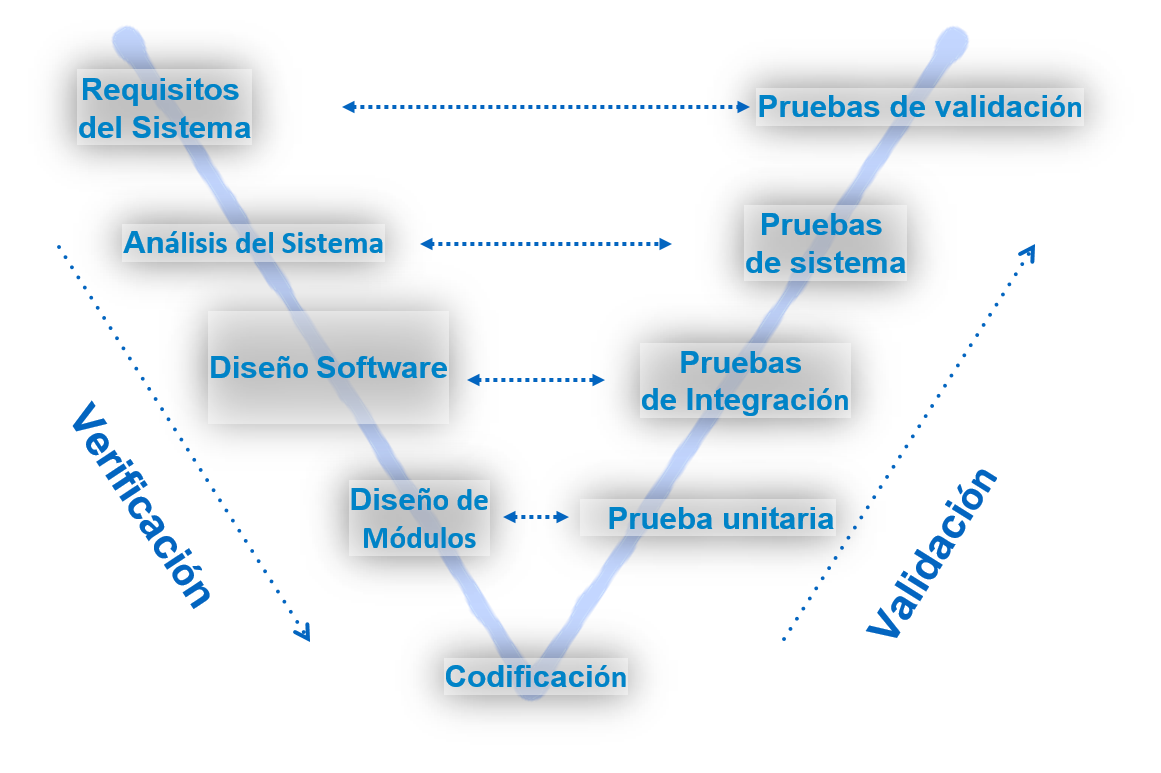
\includegraphics[scale=.5]{Capitulo3/img/vmodel.png}
	\caption{Metodología en V}
	\label{fig:ModeloIncremental}
\end{figure}

